\section{Giới thiệu dự án}

\subsection{Tổng quan}
Hệ thống điều khiển đèn giao thông là một bài toán kinh điển và thiết yếu trong hạ tầng giao thông đô thị, đòi hỏi độ tin cậy thời gian thực cao, phản hồi chính xác và đặc biệt là tính an toàn tuyệt đối nhằm ngăn ngừa xung đột giao thông. Trong khuôn khổ bài tập lớn môn Vi xử lý -- Vi điều khiển (CO3009), nhóm thực hiện thiết kế và hiện thực \textbf{``Hệ thống đèn giao thông 2 tuyến đường trên mạch XNUCLEO-F103RB''}.

Hệ thống điều khiển ngã tư giao lộ gồm 2 tuyến đường giao nhau (Tuyến 1 và Tuyến 2), sử dụng vi điều khiển STM32F103RB (lõi ARM Cortex-M3, xung nhịp hoạt động 64~MHz) trên kit phát triển XNUCLEO-F103RB cùng các thiết bị ngoại vi:
\begin{itemize}
    \item \textbf{02 module đèn giao thông}: Mỗi module đại diện cho một tuyến đường, gồm 3 đèn (Đỏ, Vàng, Xanh) được điều khiển thông qua 2 đường tín hiệu số.
    \item \textbf{04 nút nhấn chức năng}: Kết nối các chân số Arduino D7, D8, D9, D10 tương ứng với các chân GPIO của vi điều khiển, hỗ trợ chống dội và nhận diện các thao tác nhấn đơn, nhấn giữ.
    \item \textbf{01 nút nhấn USER (PC13)} trên mạch: Phục vụ chuyển đổi hoặc mở rộng chức năng hệ thống.
    \item \textbf{01 cảm biến nhiệt độ -- độ ẩm DHT20}: Giao tiếp vi điều khiển qua chuẩn I2C, cập nhật định kỳ các thông số môi trường thực tế.
    \item \textbf{01 màn hình ký tự LCD 16$\times$2 kèm module chuyển đổi I2C (PCF8574)}: Hiển thị trạng thái pha đèn, đếm ngược thời gian và thông tin nhiệt độ, độ ẩm môi trường.
\end{itemize}

\begin{figure}[!htbp]
    \centering
    \setlength{\abovecaptionskip}{8pt}
    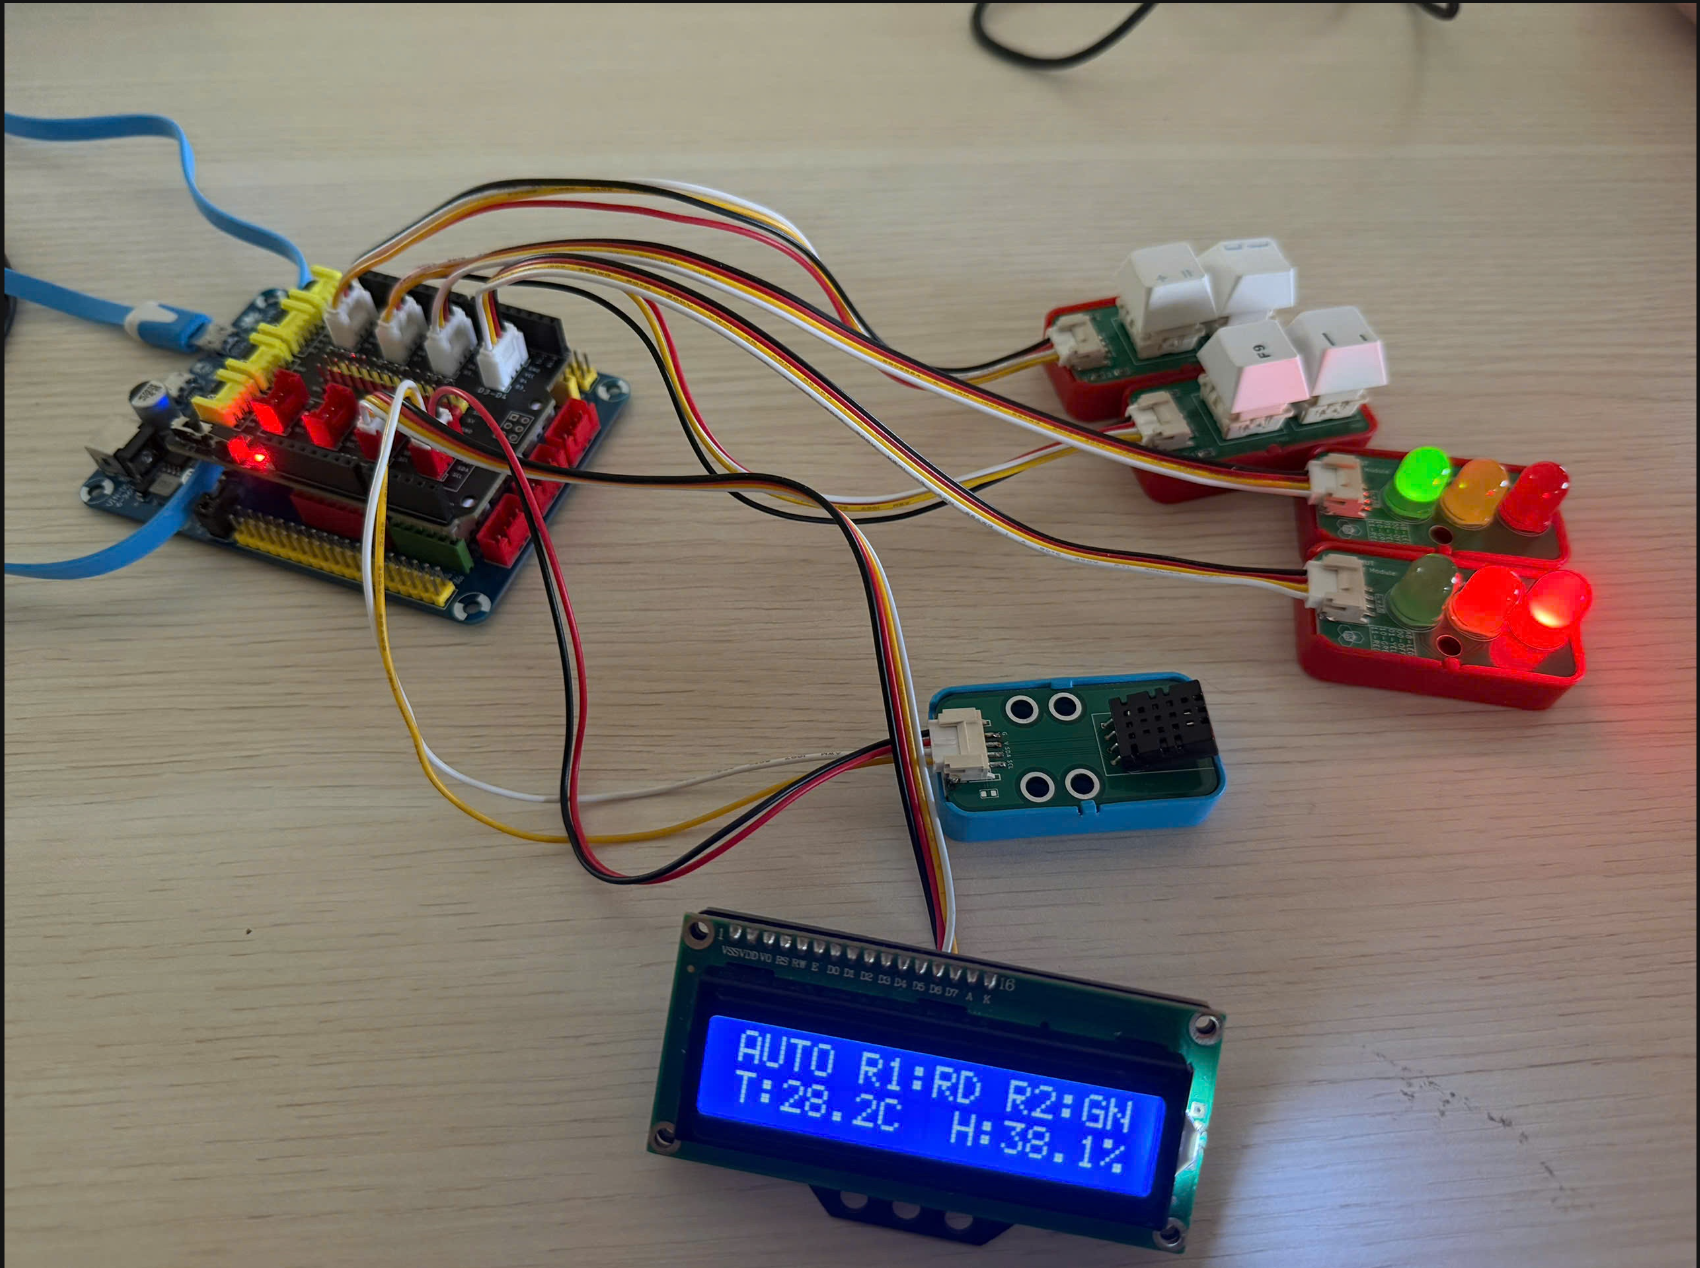
\includegraphics[width=0.75\textwidth, height=0.45\textheight, keepaspectratio]{graphics/hardware.png}
    \caption{Hệ thống phần cứng hoàn chỉnh}
    \label{fig:hardware}
\end{figure}


\subsection{Các chức năng của hệ thống}
Hệ thống cung cấp đầy đủ các chế độ vận hành theo yêu cầu của bài tập lớn, đồng thời bổ sung các cơ chế bảo vệ trạng thái an toàn:

\begin{table}[!htbp]
\centering
\footnotesize
\setlength{\tabcolsep}{4pt}
\renewcommand{\arraystretch}{1.3}
\begin{tabularx}{\textwidth}{|c|>{\raggedright\arraybackslash}p{2.3cm}|X|>{\raggedright\arraybackslash}p{3.1cm}|}
\hline
\textbf{STT} & \textbf{Chức năng} & \textbf{Mô tả chi tiết} & \textbf{Thao tác / Nút nhấn} \\ \hline
1 & \textbf{Chế độ tự động} & Điều khiển đèn giao thông 2 tuyến tuần tự theo chu kỳ Đỏ -- Xanh -- Vàng. Chèn khoảng đệm chuyển tiếp an toàn (All-Red Clearance) giữa các pha để tránh va chạm. & Tự động chạy khi khởi động; hoặc nhấn Nút 1 từ chế độ Tuning để quay về. \\ \hline
2 & \textbf{Chế độ bằng tay} & Cho phép nhân viên điều phối giao thông cưỡng bức chuyển trạng thái đèn từng bước (Manual Stepping). Trước khi cho phép một tuyến bật Xanh, tuyến đối diện bắt buộc phải chuyển về Đỏ. & Nhấn Nút 1 để vào; Nhấn Nút 2 để nhảy sang bước kế tiếp. \\ \hline
3 & \textbf{Chế độ chỉnh thời gian} & Cho phép cấu hình thời lượng đèn Đỏ, Xanh, Vàng trên màn hình LCD. Hệ thống tự động kiểm tra và chuẩn hóa quy tắc an toàn: \newline $T_{\text{Đỏ}} \ge T_{\text{Xanh}} + T_{\text{Vàng}} + 2 \times T_{\text{Clearance}}$. & Nhấn Nút 1 để vào; Nút 2: Đổi trường (R/G/Y); Nút 3: Giảm; Nút 4: Tăng. \\ \hline
4 & \textbf{Hiển thị môi trường \& LCD} & Hiển thị trạng thái pha đèn ở dòng 1 LCD; đọc cảm biến DHT20 mỗi 1 giây và hiển thị nhiệt độ, độ ẩm ở dòng 2 LCD định dạng \texttt{T:xx.xC H:xx.x\%}. & Tự động cập nhật nền qua Scheduler. \\ \hline
5 & \textbf{Chuyển chế độ an toàn} & Mỗi khi chuyển giữa các chế độ lớn (Auto $\leftrightarrow$ Manual $\leftrightarrow$ Tuning), hệ thống lập tức cưỡng bức cả 2 tuyến về Đỏ (All-Red) và reset bộ đếm thời gian. & Kích hoạt tự động khi nhấn Nút 1 (BTN\_1). \\ \hline
\end{tabularx}
\caption{Bảng tổng hợp chức năng của hệ thống}
\label{tab:system_features}
\end{table}



\subsection{Sơ đồ khối hệ thống}
